% !TeX spellcheck = en_US
\chapter{Methodology}\label{ch:method}%

This chapter presents the method. Its parts follow the three difficulties of Section~\ref{sec:problem-setup}, and each part answers one of them. Section~\ref{sec:problem} formalizes cyclic nut threading and the metrics that evaluate it. Section~\ref{sec:system} describes the simulated and physical system: the hand--arm platform, the simplified thread model that makes learning in simulation tractable (difficulty~(a)), and the action contract with its controller. Section~\ref{sec:teacher} presents the privileged reinforcement-learning teacher that learns to grasp and turn the nut with the dexterous hand (difficulty~(b)). Section~\ref{sec:hybrid} explains how the hybrid teacher chains this skill with scripted transitions into complete multi-cycle demonstrations, which is the data side of difficulty~(c), and how the pipeline prepares the student for zero-shot transfer, which is the transfer side of difficulty~(a). Section~\ref{sec:distillation} develops the central contribution, the distillation of these demonstrations into a single visuomotor student by conditional flow matching, which answers difficulty~(c) at deployment, and relates the offline and online variants. Section~\ref{sec:evaluation} defines the evaluation protocol with which Chapters~\ref{ch:sim} and~\ref{ch:real} answer RQ1 to RQ3. Figure~\ref{fig:pipeline} gives an overview.

\begin{figure}[htb]%
    \centering%
    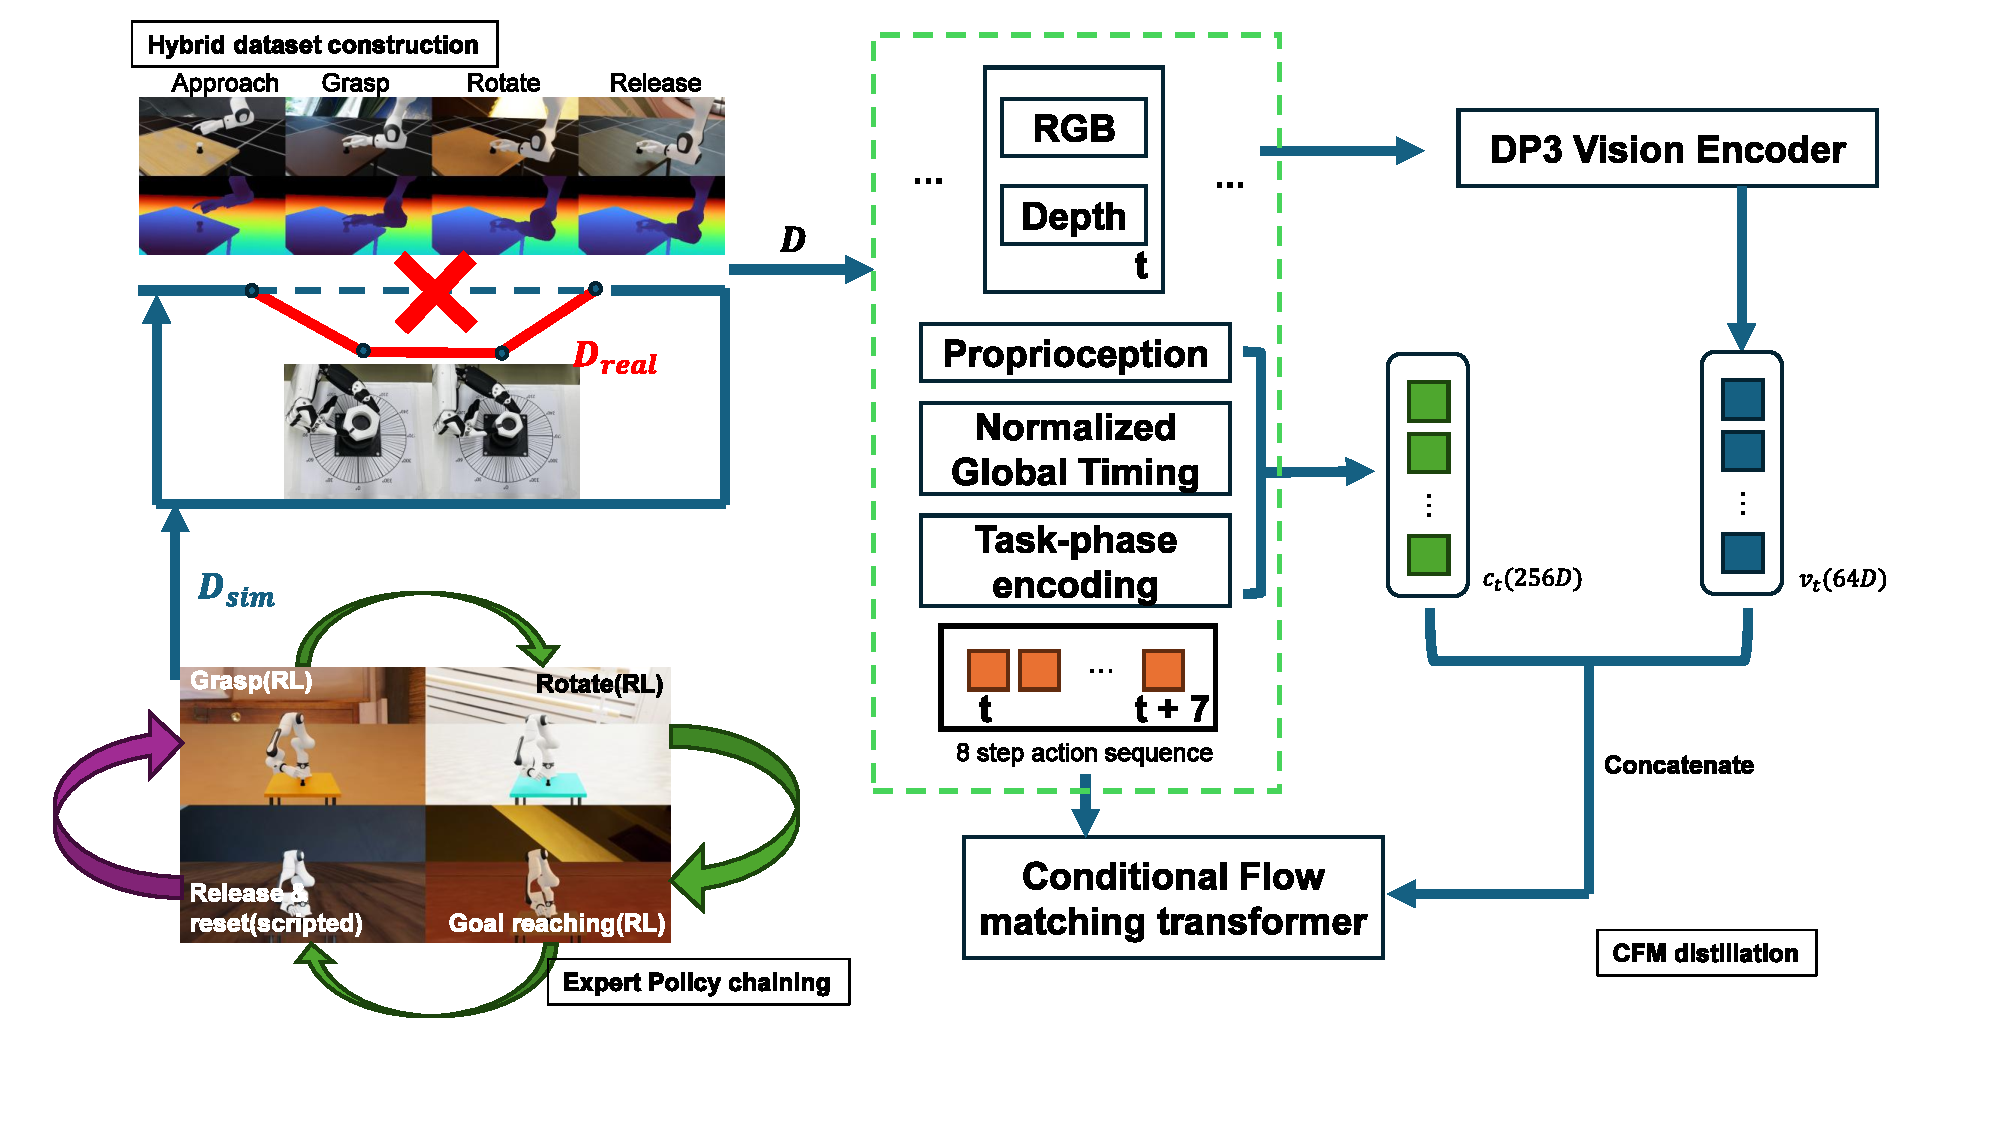
\includegraphics[width=\textwidth]{figures/mainpipeline.pdf}%
    \caption{The pipeline in detail. Left: the privileged \acs{RL} policy executes grasp, rotation, and goal reaching and a scripted controller executes release and reset; chained in a loop, they form the hybrid teacher that generates the simulated demonstrations $\Dsim$. Right: the student encodes the aligned \acs{RGBD} observation into a 64-D point-cloud feature, fuses it with proprioception, the normalized global progress, and the process-phase encoding into a 256-D condition, and a conditional flow-matching Transformer predicts an eight-step action chunk.}%
    \label{fig:pipeline}%
\end{figure}%
% TODO(figure): mainpipeline.pdf is the project's publication figure; check that it does not show the real-world replay branch with human corrections, and edit it if it does.

\section{Problem Formulation}\label{sec:problem}

Cyclic nut threading is decomposed into the ordered phase sequence
\begin{equation}\label{eq:phases}
  \mathcal{S}=\big(\underbrace{\text{approach},\;\text{grasp},\;\text{rotate},\;\text{goal reaching}}_{\MRL:\;\piT},\;\underbrace{\text{release},\;\text{return and reset}}_{\Mscript:\;\kappa}\big).
\end{equation}
The active phase at control step $t$ is $m_t\in\Mset=\MRL\cup\Mscript$. The four phases in $\MRL$ are executed by a learned teacher policy $\piT$; the two transition phases in $\Mscript$ are executed by scripted controllers $\kappa_m$. The split is a property of the data-generation stage only: the deployed student receives neither the phase label as a switch nor separate networks per phase.

Let $K$ be the required number of cycles, $\Delta\varphi^{*}$ the desired clockwise rotation per cycle, and $\varphi_k$ the unwrapped nut angle about the bolt axis after the goal-reaching phase of cycle $k$, with $\varphi_0$ the angle at the start of the trial. The cyclic tracking error, the episodic tracking error, and the tracking cost of a trajectory $\tau$ are defined as
\begin{equation}\label{eq:errors}
  e_k=\varphi_k-\varphi_{k-1}-\Delta\varphi^{*},\qquad
  e_{\mathrm{ep}}=\varphi_K-\varphi_0-K\Delta\varphi^{*}=\sum_{k=1}^{K}e_k,\qquad
  E(\tau)=\frac{1}{K}\sum_{k=1}^{K}e_k^{2}+\beta_{E}\,e_{\mathrm{ep}}^{2}.
\end{equation}
Positive errors indicate overshoot and negative errors lag; the cost squares them so that overshoot in one cycle cannot cancel lag in another, and the weight $\beta_E$ trades accumulated drift against cycle-wise accuracy. Let $C(\tau)\in\{0,\dots,K\}$ count the cycles completed before failure or timeout and let $\Pi_{\mathcal{S}}$ denote the policies that execute the phases of $\mathcal{S}$ in order in every cycle. The research problem is to find the policy that chains all phases with maximum completion success and, among those, minimum tracking cost:
\begin{equation}\label{eq:objective}
  \Pi_{\mathrm{succ}}=\argmax_{\pi\in\Pi_{\mathcal{S}}}\;\Pr_{\tau\sim p_\pi}\!\left[C(\tau)=K\right],\qquad
  \pi^{*}=\argmin_{\pi\in\Pi_{\mathrm{succ}}}\;\E_{\tau\sim p_\pi}\!\left[E(\tau)\mid C(\tau)=K\right].
\end{equation}
Throughout this thesis $K=10$ and $\Delta\varphi^{*}=60\degree$, which corresponds to one face of a hexagonal nut per cycle. The policy $\pi^{*}$ is learned from fixed hybrid-teacher demonstrations rather than by optimizing \eqref{eq:objective} on hardware, because on-robot optimization of a contact-rich cyclic task is neither safe nor sample-efficient.

The task is partially observable at deployment. The simulator state $\vec{x}_t$ contains the nut pose, the contact state, and the controller parameters; the student observes only an aligned \acs{RGBD} image, its proprioception, and two low-dimensional conditioning signals introduced in Section~\ref{sec:student}. The teacher--student structure of the method separates the two difficulties of this \ac{POMDP}: the teacher solves the control problem with privileged state, and the student learns to perceive and to reproduce the teacher's behavior from sensor data.

\section{Simulated and Physical System}\label{sec:system}

The method is trained in simulation on a model of the physical hand--arm system and deployed on that system. This section describes the platform, the thread model that makes learning in simulation tractable, and the action contract that teacher, student, and robot share.

\subsection{Platform}\label{sec:platform}

The robot is a seven-DoF torque-controlled arm with a five-fingered right hand mounted on the flange through a 10\,mm adapter; Section~\ref{sec:real-setup} names the products. The hand has twelve finger joints driven by six motors. The non-thumb fingers each have one actuated flexion joint with a mechanically coupled distal joint, and the thumb has an abduction joint and a coupled flexion chain. Only three hand degrees of freedom are commanded by the policy: thumb abduction, thumb flexion, and index flexion, which together form the pinch used for threading. The remaining fingers hold a curled posture. This restriction narrows the solution space of the dexterous hand to one grasp strategy, as difficulty~(b) of Section~\ref{sec:problem-setup} requires. The nut is threaded onto a bolt that stands on a 5\,cm pedestal on a 60\,cm by 80\,cm bench. The robot base is mounted at tabletop height, 46.5\,cm from the near table edge, so that the reach envelope lies above the work surface. A fixed \acs{RGBD} camera provides the observation; its extrinsic calibration relative to the robot base was measured on the physical cell and is reproduced in simulation.

Simulation uses Isaac~Sim~5.1 with Isaac~Lab~2.3 on the PhysX backend.
% TODO(unsure): the experiment notes record Isaac Lab 2.2.1 for the reported runs, the repository README states IsaacLab v2.3.2; confirm the version used.
Physics runs at 120\,Hz; both teacher and student act at 15\,Hz, so one policy command is held over eight physics substeps while the low-level controller closes its loop at the physics rate. The platform was selected over an earlier humanoid-arm platform on which the project started, because the present arm is substantially more precise and repeatable on the physical system. The task code, rewards, observation contracts, and training recipe are identical for both robots; only the robot asset, workcell geometry, and reset poses differ.

\subsection{Simplified Thread Simulation}\label{sec:thread-model}

The thread model is the first answer to difficulty~(a) of Section~\ref{sec:problem-setup}: the skill is learned in simulation, so the simulated thread has to be cheap enough for the thousands of parallel environments that \ac{PPO} needs. Simulating a mating thread with mesh colliders is prohibitively expensive at that scale. A kinematic thread model also gives the policy a well-posed learning signal: with \ac{SDF} thread colliders, axial progress of the nut can be obtained by pressing it along the bolt axis, whereas a kinematic coupling makes axial progress a consequence of rotation alone, so that progress can only be earned by turning. The thread model used for teacher training therefore replaces the thread contact by a kinematic coupling, illustrated in Figure~\ref{fig:thread-model}. The nut is attached to the bolt by a passive revolute joint about the bolt axis and a coaxial, position-controlled prismatic joint. With prismatic coordinate $d_t$, unwrapped and direction-corrected revolute coordinate $\theta_t$, thread pitch $\rho$, and the index $b_k$ of the step at which the current turn started, the prismatic target is
\begin{equation}\label{eq:thread}
  d^{*}_t-d_{b_k}=-\frac{\rho}{2\pi}\left(\theta_t-\theta_{b_k}\right),
\end{equation}
so that one revolution produces one pitch of axial travel. The prismatic joint tracks $d^{*}_t$ with a stiff drive (stiffness $2\times10^{5}$\,N/m, damping 200\,N\,s/m, force limit 1000\,N), whose finite stiffness permits small deviations from the ideal helix while the revolute--prismatic pair constrains lateral motion and keeps the nut near the commanded path. The finger--nut contact forces remain fully simulated: the policy must physically grip and turn the nut. Thread resistance is modeled on the revolute joint by a smoothed Coulomb and viscous friction torque
\begin{equation}\label{eq:friction}
  \bar{\tau}_{f,t}=-\tau_c\tanh\!\left(\frac{\omega_t}{\omega_s}\right)-c_v\,\omega_t,
\end{equation}
with revolute velocity $\omega_t$, Coulomb torque $\tau_c=2\times10^{-3}$\,N\,m, viscous coefficient $c_v=2\times10^{-4}$\,N\,m\,s/rad, and smoothing speed $\omega_s=0.1$\,rad/s. The nut carrier has a mass of 1\,g, and the joint limits reserve one full turn above the reset pose and a margin above the physical lower stop. The pitches are 3.0\,mm, 3.5\,mm, and 4.0\,mm for the M24, M30, and M36 nuts. The model has one deliberate simplification beyond contact: the nut is initialized already engaged with the bolt. Thread engagement from a loose nut is a separate skill with a narrow entry configuration, and it is outside the scope of this thesis. The simplified contact opens a gap between the simulated and the physical thread, which the transfer design of Section~\ref{sec:sim2real} has to bridge.

\begin{figure}[htb]%
    \centering%
    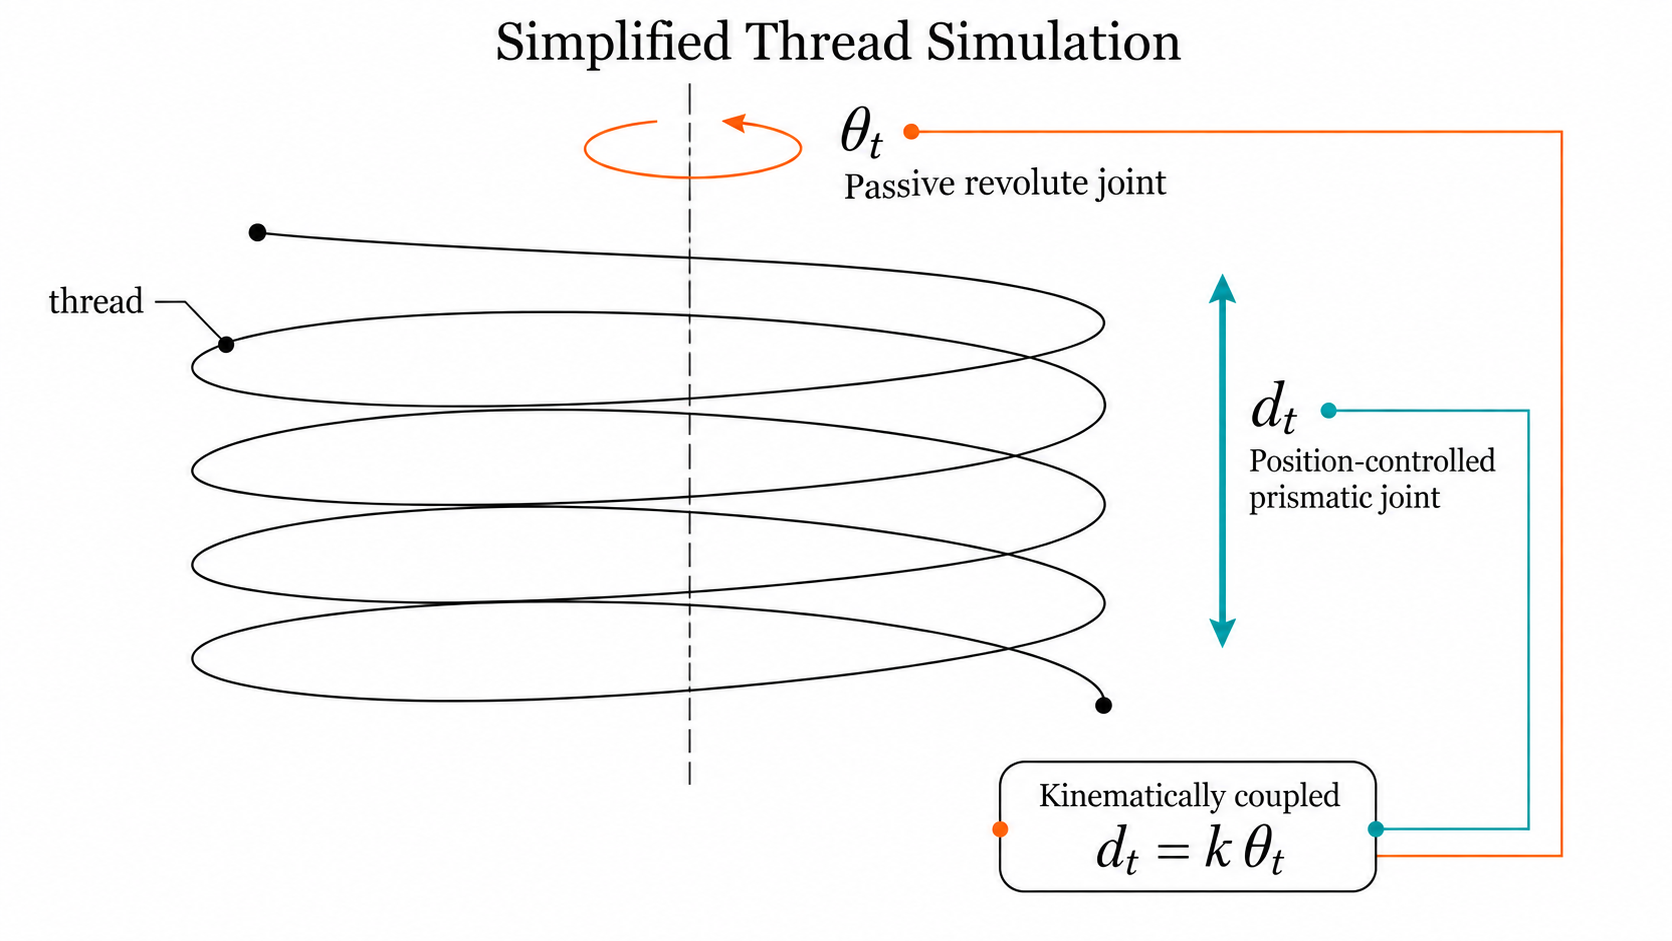
\includegraphics[width=0.62\textwidth]{figures/simplified_thread_simulation-v3.png}%
    \caption{Simplified thread simulation. A passive revolute joint $\theta_t$ about the bolt axis is kinematically coupled to a position-controlled prismatic joint $d_t$ through $d_t=k\theta_t$ with $k=-\rho/(2\pi)$, so that the nut advances by one pitch per revolution without explicit thread contacts; the finger--nut contacts remain fully simulated.}%
    \label{fig:thread-model}%
\end{figure}%

\subsection{Action Contract and Controller}\label{sec:action-contract}

Teacher and student share one action space, a 9-D vector $\vec{a}_t\in[-1,1]^9$ that is decoded into a Cartesian target for the hand's grasp frame and three pinch-joint targets. The grasp frame is a fixed offset from the flange whose origin lies at the thumb--index pad midpoint, whose $z$ axis points along the approach direction, and whose $x$ axis is the pinch-closing axis. The first three components scale by 0.05\,m to a position offset relative to an action frame that is the bolt tip during threading and the held nut during pickup; because the target is expressed relative to the bolt, the controller draws the grasped nut toward the bolt regardless of where nut and robot are, and a zero action does not hold the current pose. Components four to six set the orientation: roll and pitch scale by 1\,rad around a neutral grasp orientation, and yaw maps $[-1,1]$ to the window $[-180\degree,90\degree]$ inside the wrist joint limits. Components seven to nine command the thumb abduction, thumb flexion, and index flexion joints, where zero holds the closed-grasp posture and $\pm1$ moves by half the admissible joint range. The raw action is smoothed by an exponential moving average with factor sampled per episode from $[0.025,0.1]$ (three times larger, capped at one, for the fingers), and the resulting target is clipped to at most 0.02\,m and 0.097\,rad from the current pose per step, so that one command cannot demand a large jump.

The Cartesian target is tracked by the task-space impedance controller of \eqref{eq:osc}, inherited from Factory and FORGE, with proportional gains $[565,565,565,28,28,28]$ (N/m and N\,m/rad), critical damping, a nullspace posture term with gains $10$ and $6.32$, and a dead zone of $[5,5,5,1,1,1]$ (N and N\,m) below which wrench components are zeroed. The gains act component-wise in world axes, so the impedance ellipsoid is aligned with the vertical bolt axis. The arm's own joint drives are disabled and the controller output is applied as joint torque; the finger joints are position-controlled by the simulator's implicit \acs{PD} drives. For training robustness and for sim-to-real transfer, the controller parameters are randomized per episode: gains by a multiplicative factor in $[1/1.41,1.41]$, position and rotation thresholds by $\pm25\%$ and $\pm29\%$, and the dead zone by uniform resampling every two seconds. The critic observes the sampled values, the actor does not.

For deployment, the same controller law is reproduced on the physical arm in a Cartesian impedance controller that uses the quaternion-vector orientation error, a damped pseudoinverse for the nullspace projector, and the robot's own gravity and Coriolis compensation; the gains of the physical controller are documented in Chapter~\ref{ch:real}. The shared Cartesian action space for teacher, student, and robot results from a design decision, and the decision is recorded here because the project also implemented and evaluated an alternative. The alternative, called the 17-D impedance joint-PD contract, has the student emit seven arm position references, seven arm velocity references, and three pinch positions, which a joint-space impedance controller tracks as
\begin{equation}\label{eq:pd}
  \vec{\tau}=\vec{g}(\vec{q})+\mat{K}_p^{\mathrm{hw}}\left(\vec{q}_{\mathrm{ref}}-\vec{q}\right)+\mat{K}_d^{\mathrm{hw}}\left(\dot{\vec{q}}_{\mathrm{ref}}-\dot{\vec{q}}\right),
\end{equation}
with gravity compensation $\vec{g}(\vec{q})$ owned by the controller. Teacher labels are converted to this contract by evaluating the Cartesian controller and reverse-engineering the equivalent joint references, $\vec{q}_{\mathrm{ref}}=\vec{q}+(\mat{K}_p^{\mathrm{hw}})^{-1}\vec{\tau}_{\mathrm{OSC}}$ and $\dot{\vec{q}}_{\mathrm{ref}}=\dot{\vec{q}}$. The motivation was that a joint-space command is the native interface of most robot drivers. Replaying recorded 17-D commands at the physics rate reproduced the teacher motion with an arm-joint \acs{RMSE} of 0.0037\,rad, so the controller itself is adequate. The contract is nevertheless unfavorable for learning, for three reasons. First, the equivalent joint target changes within the eight physics ticks over which a 15\,Hz student command is held, so a zero-order hold introduces a target error of 0.010 to 0.015\,rad and an implied torque error of up to 16\,N\,m. Second, the commands are in physical units with widely different scales across the 17 dimensions. Third, as Chapter~\ref{ch:sim} reports, only students trained on the Cartesian contract reach the task goals in closed loop. The Cartesian contract, in which the student imitates the bounded, bolt-relative action that the teacher itself produced and executes it through the unchanged controller, removes this conversion and is the contract of all reported results. The 17-D contract is retained as an ablation.

\section{Privileged Teacher Training}\label{sec:teacher}

The privileged teacher answers difficulty~(b) of Section~\ref{sec:problem-setup}. It learns to approach the nut, acquire the pinch grasp, keep it under load while turning, and hold the target, all through the commanded hand and arm degrees of freedom of Section~\ref{sec:platform}. Because it observes privileged simulator state, it solves this control problem without having to perceive the nut (Section~\ref{sec:problem}).

The teacher for the learned phases in $\MRL$ is a recurrent policy trained with \ac{PPO} in an asymmetric actor--critic. The actor observation $\vec{z}^{\pi}_t=g_\pi(\vec{x}_t,\vec{\xi}_t)$ selects the actor-visible components of the simulator state and applies observation noise $\vec{\xi}_t$; it comprises the fingertip (grasp-frame) position relative to the bolt frame and its quaternion, the end-effector linear and angular velocity obtained by finite differences, the fingertip position relative to the held nut and the nut quaternion, the position and quaternion error to the current turning target, a grasp-phase flag that indicates whether the proper grasp has latched, the previous filtered action, and, for the multi-size teacher, a one-hot code of the nut size. Position terms receive Gaussian noise with 0.25\,mm standard deviation per axis, orientation terms 0.1\degree, and the bolt frame a per-episode offset of 1\,mm, which models calibration error. The critic observes the same task and history structure using clean values and extends it with the arm joint positions, the complete nut and bolt pose, the sampled controller gains, smoothing factor, and thresholds, and the thumb and index contact forces. Table~\ref{tab:teacher-obs} in the appendix lists the exact components and widths.

Actor and central critic share the same architecture: a two-layer \ac{LSTM} with 1024 units per layer and layer normalization, followed by a 512--128--64 \acs{MLP} with ELU activations. Recurrent sequences span 128 control steps, the rollout horizon is 256 steps, and the actor parameterizes a diagonal Gaussian over the normalized action with a state-dependent standard deviation. The teacher is optimized with the shaped reward
\begin{equation}\label{eq:reward}
\begin{aligned}
  r_t&=\sum_{i\in\mathcal{R}} w^{r}_{i}R_{i,t}-\sum_{j\in\mathcal{P}} w^{p}_{j}P_{j,t},\\
  \mathcal{R}&=\{\text{center},\text{face},\text{grasp},\text{turn},\text{target}\},\qquad
  \mathcal{P}=\{\text{mag},\Delta a,\text{align},\text{force},\text{settle},\text{clear},\text{contact}\}.
\end{aligned}
\end{equation}
The reward follows the three phases of the learned behavior. During approach, $R^{\mathrm{center}}$ rewards motion of the grasp center toward the nut center and $R^{\mathrm{face}}$ rewards motion of the thumb and index pads toward the two designated opposing faces of the nut; both pay $20$ times the newly achieved fraction of the initial gap, so repeated motion cannot accumulate reward. $R^{\mathrm{grasp}}$ pays a one-time bonus of $100$ when a proper grasp, defined as simultaneous thumb and index contact on the designated faces with a pinch line perpendicular to the nut axis, has held for five consecutive steps. During turning, $R^{\mathrm{turn}}$ pays $60$ times the newly achieved fraction of the distance to the fixed helical target pose, and pays only while the previously acquired proper grasp remains live. At completion, $R^{\mathrm{target}}$ pays $250$ distributed over a five-step hold within $5\degree$ of the target. The penalties discourage large commands ($P^{\mathrm{mag}}$, weight $10^{-3}$), abrupt action changes ($P^{\Delta a}$, $0.1$), misalignment of the hand frame with the nut frame ($P^{\mathrm{align}}$, $0.02$), excess wrist force ($P^{\mathrm{force}}$, $0.05$), residual rotation near the target ($P^{\mathrm{settle}}$, $0.25\,\omega_t^2$ from $50\degree$ onward), insufficient table clearance ($P^{\mathrm{clear}}$), and arm--table contact ($P^{\mathrm{contact}}$). An episode succeeds when at least $55\degree$ of clockwise rotation is held with a live proper grasp for five steps; it terminates early when the nut leaves the bolt by more than 3\,cm, tilts by more than $60\degree$, or releases the thread, and when the grasp is lost after it has latched. The last rule turns grasp retention into a hard constraint rather than a shaped term.

Robustness is obtained by domain randomization of the nut mass ($\pm5$\,g), the bolt friction (static coefficient in $[0.25,1.25]$), the controller parameters of Section~\ref{sec:action-contract}, and the initial state; Table~\ref{tab:dr} lists the ranges. The observation noise is small in absolute terms, a quarter of a millimeter and a tenth of a degree, because the actor's inputs are relative poses that the student will later infer from a calibrated camera; the per-episode bolt-frame offset of one millimeter is the term that models calibration error and forces the teacher to close the loop on the nut rather than on the bolt frame. The initial nut rotation is randomized by an automatic curriculum: the yaw range starts at zero and expands by $5\degree$ whenever the population success rate exceeds 80\,\%, up to $\pm30\degree$, with at least five episode lengths between expansions; the initial axial height is sampled uniformly up to 20\,mm below the nominal spawn while reserving room for the full $60\degree$ target turn. \begin{table}[htb]%
    \centering%
    \caption{Domain randomization during teacher training. $U(a,b)$ denotes uniform sampling; multiplicative factors are sampled as $1+U(0,\ell)$ or its reciprocal with equal probability.}%
    \label{tab:dr}%
    \small
    \begin{tabular}{lll}
        \toprule
        Group & Quantity & Range \\
        \midrule
        physics & nut mass offset & $U(-5,5)$\,g per reset \\
         & bolt static friction & $U(0.25,1.25)$, 128 buckets \\
        controller & proportional gains & multiplicative, $\ell=0.41$, per axis and reset \\
         & action smoothing factor & $U(0.025,0.1)$ per reset; fingers $3\times$ \\
         & position / rotation threshold & multiplicative, $\ell=0.25$ / $0.29$ \\
         & dead zone & $U(0,[5,5,5,1,1,1])$ N, N\,m, resampled every 2\,s \\
        observation & fingertip and nut position & $\mathcal{N}(0,0.25\,\mathrm{mm})$ per axis and refresh \\
         & fingertip and nut orientation & random-axis angle $\mathcal{N}(0,0.1\degree)$ \\
         & bolt frame & $\mathcal{N}(0,1\,\mathrm{mm})$ per axis and reset \\
         & fingertip forces & $\mathcal{N}(0,1\,\mathrm{N})$ per channel \\
        initial state & nut yaw & curriculum $0\rightarrow\pm30\degree$ in $5\degree$ steps at 80\,\% success \\
         & nut axial height & $U(0,20)$\,mm below nominal, full turn reserved \\
         & nut size & round-robin M24 / M30 / M36 (multi-size teacher) \\
        \bottomrule
    \end{tabular}
\end{table}%

A single teacher is conditioned on the M24, M30, and M36 nuts through the one-hot code and round-robin assignment of sizes to environments. Training uses 512 parallel environments for 200 epochs and takes about ten hours on one NVIDIA GeForce RTX~5090; the \ac{PPO} hyperparameters are listed in Table~\ref{tab:ppo} in the appendix.

A second expert, the pickup teacher, was trained with the same recipe for grasping a loose nut from the table, lifting it, transporting it to a handoff pose above the bolt tip, and engaging it; its reward uses the same approach and grasp terms, a lift term, and keypoint progress toward two waypoints. It is part of the full-task variant of the hybrid teacher described below and is reported for completeness in Chapter~\ref{ch:sim}; it is not part of the final threading pipeline, whose trials start from an engaged nut.

\section{Hybrid Teacher and Demonstration Generation}\label{sec:hybrid}

The privileged teacher turns the nut once. The hybrid teacher answers the data side of difficulty~(c) of Section~\ref{sec:problem-setup}: it chains the learned turn with scripted release and return, so that each phase is specified by the mechanism that specifies it most simply, and it rolls the chain out in simulation to produce complete multi-cycle demonstrations. This section describes the cyclic rollout, its full-task variant, the disturbance augmentation, and the dataset. It also collects the design choices that answer the transfer side of difficulty~(a) (Section~\ref{sec:sim2real}), because most of them are fixed when the demonstrations are rendered.

\subsection{Cyclic Teacher Rollout in Simulation}\label{sec:hybrid-rollout}

Let $m_t\in\Mset$ denote the active phase, $\vec{x}_t$ the full simulator state, $\vec{z}^{\pi}_t$ the noisy actor observation, and $\vec{h}_t$ the actor's recurrent state. During rollout the teacher is queried for its deterministic mean action $\bar{\pi}_{\mathrm{T}}(\vec{z}^{\pi}_t,\vec{h}_t)=\E_{\vec{a}\sim\piT(\cdot\mid\vec{z}^{\pi}_t,\vec{h}_t)}[\vec{a}]$. The hybrid teacher is
\begin{equation}\label{eq:hybrid}
  \piHT(\vec{x}_t,m_t)=
  \begin{cases}
    \bar{\pi}_{\mathrm{T}}(\vec{z}^{\pi}_t,\vec{h}_t), & m_t\in\MRL,\\
    \kappa_{m_t}(\vec{x}_t), & m_t\in\Mscript,
  \end{cases}
\end{equation}
where $\kappa_{m_t}$ is the scripted controller of the active transition phase. Both branches produce commands in the same filtered, bolt-relative Cartesian action space, so the recorded label is a single 9-D signal throughout the cycle; the scripted Cartesian targets are inverse-decoded through the action mapping of Section~\ref{sec:action-contract}, and the executing adapter compensates the action smoothing analytically so that the controller receives exactly the requested target. This unified label space is what makes the demonstration a coherent supervision signal for one student: at no step does the label change meaning or units.

Release is triggered when the nut rotation lies within $\pm5\degree$ of the $60\degree$ target while a valid opposed-finger grasp has been maintained for a short dwell. The fingers then open to a safe clearance, after which four Cartesian waypoints retract the hand along the ray from the nut center through the grasp center, raise it, and return it to the initial grasp pose. Each waypoint segment is interpolated over 0.7\,s and the final return over 1.0\,s; the return is physically gated and counts as complete only when the grasp frame is within 5\,mm and $5\degree$ of the reset frame and the hand joints within 0.15\,rad of their reset values, with a 16\,s timeout that marks the cycle as a transition failure. The waypoints were authored once by a collision-safe retargeting from a captured release pose and verified to produce zero pad--nut contact force during every release. While the hand is away from the nut the thread joint is held, so the nut cannot drift between cycles. On a completed return the turning reference is rebased: the target angle advances by $60\degree$ relative to the current nut pose, the frozen threading policy receives a cycle-local canonicalized nut orientation so that it sees the same observation statistics in every cycle, and its recurrent state and action history are reseeded. The physical nut pose is not reset, so the demonstration contains the axial advance of the nut over ten cycles. The teacher population was first qualified for one period only; repeated cycles are a property of the hybrid rollout, not of the \ac{RL} teacher alone. Figure~\ref{fig:datacollection} shows the coordinator that sequences one cycle.

Two details of the coordinator matter for the quality of the labels. First, the scripted transitions never write physics state: a transition may request that the thread joint be held while the hand is away, but it repairs nothing by teleporting the nut, so every recorded frame is a physically consistent consequence of the recorded commands; an earlier implementation that snapped the nut back at the policy rate produced visible reversals of the nut at release that the student would have imitated. Second, the release gate is physical rather than timed: release is decided from the measured nut rotation and the measured grasp, and the return is validated against the reset frame, so the phase labels in the recording coincide with physical events. Both properties are what allow the recorded phase to be used as a conditioning signal at deployment, where it is derived from the same physical events.

\begin{figure}[htb]%
    \centering%
    % Hybrid-teacher data-collection loop (cyclic coordinator).
\resizebox{\textwidth}{!}{%
\begin{tikzpicture}[
  font=\small,
  state/.style={draw, rounded corners=3pt, align=center, minimum height=10mm, inner sep=4pt, fill=white, text width=30mm},
  rl/.style={state, fill=TUMBlue!12},
  sc/.style={state, fill=TUMOrange!15},
  gate/.style={draw, diamond, aspect=2.2, align=center, inner sep=1pt, fill=white, font=\footnotesize},
  arr/.style={-{Latex[length=2mm]}, thick},
  node distance=6mm and 9mm,
]
\node[rl] (policy) {threading policy $\bar{\pi}_{\mathrm{T}}$\\approach, grasp, turn, hold};
\node[gate, right=of policy] (relgate) {$\Delta\varphi\ge55\degree$?};
\node[sc, right=of relgate] (waypoints) {four Cartesian waypoints,\\0.7\,s each: open pinch,\\retreat, lift\\(thread joint held)};
\node[sc, below=of waypoints] (return) {return to\\reset pose, 1.0\,s};
\node[gate, left=of return] (retgate) {within 5\,mm, $5\degree$,\\0.15\,rad?\\(16\,s timeout)};
\node[state, left=of retgate, fill=TUMGreen!15] (rebase) {rebase: target $+60\degree$,\\canonical nut frame,\\reseed $\vec{h}$, cycle $k{+}1$};
\node[state, below=of policy, fill=red!10, text width=30mm] (fail) {transition failure:\\episode rejected};
\draw[arr] (policy) -- (relgate);
\draw[arr] (relgate) -- node[above, font=\footnotesize] {yes} (waypoints);
\draw[arr] (relgate.south) |- node[pos=0.75, below, font=\footnotesize] {no: keep turning} ++(-10mm,-6mm) -| (policy.south east);
\draw[arr] (waypoints) -- (return);
\draw[arr] (return) -- (retgate);
\draw[arr] (retgate) -- node[above, font=\footnotesize] {yes} (rebase);
\draw[arr] (retgate.south) |- node[pos=0.75, below, font=\footnotesize] {no} (fail.east);
\draw[arr] (rebase.west) -| node[pos=0.25, below, font=\footnotesize] {$k<K$} (policy.south);
\node[above=3mm of relgate, font=\footnotesize, align=center, text width=100mm] {every segment receives one random arm impulse (0.05--0.25\,N\,s); every executed command is recorded as the 9-D label together with RGB-D, proprioception, progress, and phase};
\end{tikzpicture}%
}
%
    \caption{Data-collection loop of the hybrid teacher for one threading cycle. The learned policy owns approach, grasp, turn, and hold; a physical release gate hands over to the scripted release, four retreat waypoints, and the gated return; a completed return rebases the turning target and starts the next cycle. Every executed command is recorded in the common 9-D label space.}%
    \label{fig:datacollection}%
\end{figure}%

\subsection{Full-Task Variant with Pickup and Handover}\label{sec:hybrid-fulltask}

The hybrid teacher also has a full-task variant that prepends the pickup expert and a scripted pickup-to-threading handover (open the hand, move to the threading reset pose, close, settle, with phase durations of 0.4, 1.5, 0.4, and 0.25\,s) to the cyclic threading teacher. The resulting demonstrations start from a loose nut on the table. Both variants and their single-phase special cases (pickup only, one threading turn, cyclic threading) are selected by one training-environment option and expose the same supervision contract, so that a student trained on either variant can be evaluated with the same tools. Because thread engagement is outside the scope of this thesis (Section~\ref{sec:thread-model}), the reported threading results use the cyclic variant from an engaged nut.

\subsection{Disturbance Augmentation}\label{sec:impulses}

Twenty demonstrations contain too little variation for a student that must recover from its own deviations. Trajectory diversity is therefore increased at collection time by applying random impulses to the arm: in every contiguous teacher-phase segment, that is, in every policy, waypoint-following, and return segment of every cycle, one impulse with a magnitude of 0.05 to 0.25\,N\,s is applied to a random arm link between 0.05 and 0.20\,s after the segment begins, giving 30 impulses per ten-cycle demonstration. The teacher, which is a closed-loop controller, reacts to the disturbance, and the recorded recovery is part of the label. Because the teacher runs deterministically at $\beta=1$ with the disturbance as the only source of variation, the recovery segments remain consistent with the trajectory that conditions them. Demonstrations in which the teacher fails to complete all cycles are rejected before materialization; the retained set consists only of explicitly successful episodes.

\subsection{Zero-Shot Sim-to-Real Transfer}\label{sec:sim2real}

The student is trained on the simulated demonstrations alone, $\Dset=\Dsim$, and deployed on the physical robot without real-world training data. Section~\ref{sec:thread-model} answered the simulation side of difficulty~(a); this subsection answers its transfer side. The simplified thread model and the rendered images open a gap in contact and perception between the two domains, and four properties of the pipeline are designed to carry the student across it. RQ3 asks whether they suffice, and Chapter~\ref{ch:real} tests it.

The first is a shared camera model. The extrinsic pose of the physical camera relative to the robot base is measured on the physical cell by an eye-to-hand calibration, and the calibrated pose and intrinsics are used to render the simulated camera; the $640\times480$ stream is center-cropped to $640\times360$ and downscaled by two in both domains, with the intrinsics scaled accordingly. Simulated and real point clouds are therefore expressed in the same frame and have the same resolution and field of view.

The second is a metric representation. The student encodes a point cloud back-projected from the depth image (Section~\ref{sec:student}), not the image itself. Points are kept only inside a fixed crop box around the workspace and within a valid depth range, so that the background, which differs most between the rendered and the physical scene, never enters the representation, and the geometry of nut, bolt, and hand is identical in both domains up to depth noise and calibration error. Random sampling of 4096 points per frame during training acts as an additional augmentation of the point set.

The third is visual domain randomization at collection time. The demonstrations are rendered with randomized dome lighting, tabletop texture, nut and bolt textures, floor texture, and image background in the style of DextrAH-RGB~\cite{Singh2025}, each component switchable individually. Because the offline loader cannot regenerate scene appearance from stored images, this variation is recorded into the dataset once and reused unchanged by every student trained on it. During training, the stored RGB images are further perturbed by saturation, contrast, and brightness factors in $[0.5,1.5]$, hue shifts in $[-0.15,0.15]$, and motion blur with probability 0.1. The depth channel is not modified by the offline trainer; the encoder pretraining of Section~\ref{sec:student} provides a depth-corruption model of a commodity \acs{RGBD} sensor with Gaussian and range-dependent axial noise, low-frequency spatial noise, millimeter quantization, dropout at depth discontinuities, correlated missing regions, and uniform dropout.
% TODO(unsure): confirm which depth-noise model (none, gaussian, realistic) the sweep pretraining of the retained DP3 encoder used.

The fourth is a shared action path. The student imitates the teacher's bounded, bolt-relative Cartesian action, and on the physical robot this action is executed by a Cartesian impedance controller that reproduces the simulated control law (Section~\ref{sec:action-contract}). The teacher itself was trained under randomized controller gains, smoothing factors, and dead zones and under noise on every pose input (Table~\ref{tab:dr}), so the behavior that the demonstrations record is robust to the controller and calibration deviations that the physical system introduces.
% TODO(results): measure real depth failures, exposure, blur, and camera/control latency on the physical camera and set the simulation randomization ranges from them (forgeUltra todo.md, P2).

\subsection{Dataset Format}\label{sec:dataset}

Each demonstration is materialized as one episode file with aligned 15\,Hz samples. A sample holds the RGB image and the metric depth image at $320\times180$ pixels, obtained by center-cropping the $640\times480$ camera stream to $640\times360$ and downscaling by two with the intrinsics scaled accordingly; the 29-D proprioception, consisting of the ten controlled joint positions, their velocities, and the previous filtered 9-D action; the executed 9-D command; the normalized task progress; the active process phase; the nut pose for privileged ablations and auxiliary supervision; and the timestamp. The recorder stores the 17-D joint-PD equivalent of every command alongside, so that both action contracts can be trained from one collection. Chunks that cross a physical reset are masked, phase boundaries are retained so that the student learns the transitions, and terminal chunks are padded with the final valid command so that the last observations of an episode remain conditioning states. For the retained M24 dataset, 20 successful ten-cycle demonstrations collected from 32 parallel environments contain 19\,486 frames.

\section{Student Policy Distillation by Conditional Flow Matching}\label{sec:distillation}

The student answers the deployment side of difficulty~(c) of Section~\ref{sec:problem-setup}. The hybrid teacher cannot be deployed, because both its learned policy and its scripted controllers act on privileged simulator state \eqref{eq:hybrid}. The student replaces it with one visuomotor policy that executes every phase of every cycle from sensor data, without a phase switch or separate networks. RQ1 asks whether this unified student sustains consecutive cycles better than a single-cycle policy invoked repeatedly. RQ2 asks which student design distills the demonstrations best; the alternative encoders of Section~\ref{sec:student} and the regression baselines of Section~\ref{sec:baselines} are its comparisons.

\subsection{From Behavior Cloning to Online Distillation for Cyclic Tasks}\label{sec:why-dagger}

Student learning is posed as supervised imitation from the fixed dataset $\Dset$. Section~\ref{sec:il-background} explained why plain behavior cloning is fragile over long horizons: the student is evaluated on the states that its own errors produce. For cyclic threading the mechanism is concrete. A student that grasps a millimeter too high applies a slightly different torque, the nut advances a little less, and after a few cycles the fingers close on the edge of the nut instead of on its faces. Three measures counter this compounding in the present method, and they are complementary. First, the demonstrations themselves contain recoveries, because the closed-loop teacher was disturbed by impulses during collection; the student thus sees off-nominal states with correct labels, which is the effect \ac{DAgger} produces by querying the expert on student-visited states, obtained here without an expert that can be queried at arbitrary states. Second, the student predicts action chunks and executes a temporal ensemble of overlapping chunks, which filters the single-step noise that would otherwise be amplified by the controller. Third, where a queryable expert exists, in simulation, the same flow-matching student can be trained online with the hybrid teacher labeling the states that the student visits; this online variant is described in Section~\ref{sec:online-flow} and compared with the offline variant in Chapter~\ref{ch:sim}. The deployed student is trained offline on $\Dset$: the dataset is rendered once under visual randomization and reused unchanged by every student and ablation, and the offline flow student sustains ten cycles (Chapter~\ref{ch:sim}). Online \ac{DAgger} serves as a comparison in simulation.

\subsection{Flow Matching for Conditional Action Chunks}\label{sec:flow-matching}

Flow matching learns a generative model as the solution of an \ac{ODE}. Let $\vec{x}\in\R^{d}$ denote a sample, let $p_0=\mathcal{N}(\vec{0},\mat{I})$ be the source distribution, and let $p_1=q$ be the data distribution. A time-dependent vector field $\vec{v}:\R^{d}\times[0,1]\to\R^{d}$ defines a flow $\psi_\lambda$ through $\frac{\mathrm{d}}{\mathrm{d}\lambda}\psi_\lambda(\vec{x})=\vec{v}(\psi_\lambda(\vec{x}),\lambda)$ with $\psi_0(\vec{x})=\vec{x}$, and the flow transports $p_0$ to the marginal path $p_\lambda=[\psi_\lambda]_{\#}p_0$. The flow-matching objective regresses a parametric field $\vfield$ onto a target field $\vec{u}_\lambda$ that generates a prescribed path $p_\lambda$ from $p_0$ to $p_1$:
\begin{equation}\label{eq:fm}
  L_{\mathrm{FM}}(\theta)=\E_{\lambda\sim U[0,1],\,\vec{x}\sim p_\lambda}\left\|\vfield(\vec{x},\lambda)-\vec{u}_\lambda(\vec{x})\right\|_2^{2}.
\end{equation}
This objective cannot be evaluated directly, because the marginal path and its field are defined only implicitly by the data. Conditional flow matching~\cite{Lipman2023} resolves this by constructing the marginal path as a mixture of conditional paths $p_\lambda(\vec{x}\mid\vec{x}^{1})$, one per data sample $\vec{x}^{1}\sim q$, each with a known conditional field $\vec{u}_\lambda(\vec{x}\mid\vec{x}^{1})$. The marginal field is the posterior-weighted average of the conditional fields,
\begin{equation}\label{eq:marginal-field}
  \vec{u}_\lambda(\vec{x})=\int\vec{u}_\lambda(\vec{x}\mid\vec{x}^{1})\,\frac{p_\lambda(\vec{x}\mid\vec{x}^{1})\,q(\vec{x}^{1})}{p_\lambda(\vec{x})}\,\mathrm{d}\vec{x}^{1},
\end{equation}
and the conditional objective
\begin{equation}\label{eq:cfm}
  L_{\mathrm{CFM}}(\theta)=\E_{\lambda\sim U[0,1],\,\vec{x}^{1}\sim q,\,\vec{x}\sim p_\lambda(\cdot\mid\vec{x}^{1})}\left\|\vfield(\vec{x},\lambda)-\vec{u}_\lambda(\vec{x}\mid\vec{x}^{1})\right\|_2^{2}
\end{equation}
has the same gradient with respect to $\theta$ as \eqref{eq:fm}; the two differ only by a constant that does not depend on $\theta$, which follows by expanding the squares and using \eqref{eq:marginal-field}. The conditional path can therefore be chosen for convenience. The optimal-transport path takes the conditional distribution to be Gaussian with mean $\lambda\vec{x}^{1}$ and standard deviation $1-\lambda$ (up to a small floor), so that a sample is the straight-line interpolant
\begin{equation}\label{eq:interpolant}
  \vec{x}^{\lambda}=(1-\lambda)\vec{x}^{0}+\lambda\vec{x}^{1},\qquad \vec{x}^{0}\sim p_0,
\end{equation}
and the conditional field along this line is constant, $\vec{u}_\lambda(\vec{x}^{\lambda}\mid\vec{x}^{1})=\vec{x}^{1}-\vec{x}^{0}$. Straight conditional paths make the learned marginal field nearly straight as well, which is why few integration steps suffice at sampling time.

The student applies this construction to action chunks conditioned on the observation. At control step $t$ the student observes $\obs_t=(\vec{O}^{\mathrm{RGBD}}_t,\vec{s}_t,p_t,\vec{e}^{m}_t)$, consisting of the \acs{RGBD} image, the proprioception $\vec{s}_t$, the normalized task progress $p_t$, and the process-phase encoding $\vec{e}^{m}_t$, and learns the distribution of the executed $H$-step action chunk. The supervision target is the demonstrated chunk $\Uc^{D}_t=[\act_t,\dots,\act_{t+H-1}]\in\R^{H\times9}$, the observation is encoded into a condition vector $\cond_t$ by the network of Section~\ref{sec:student}, and the distillation objective is
\begin{equation}\label{eq:student-objective}
  \theta^{*}=\argmin_\theta\;\E\left\|\vfield\!\left(\Uc^{\lambda}_t,\lambda\mid\cond_t\right)-\dot{\Uc}^{\lambda}_t\right\|_2^{2},\qquad
  \Uc^{\lambda}_t=(1-\lambda)\Uc^{0}_t+\lambda\Uc^{D}_t,\quad
  \dot{\Uc}^{\lambda}_t=\Uc^{D}_t-\Uc^{0}_t,
\end{equation}
where the expectation is over $(\obs_t,\Uc^{D}_t)\sim\Dset$, $\Uc^{0}_t\sim\mathcal{N}(\vec{0},\mat{I})$, and $\lambda\sim U[0,1]$. The learned field transports Gaussian noise to the conditional action distribution $p_\theta(\Uc_t\mid\obs_t)$. At inference, a chunk is generated by drawing $\Uc^{0}\sim\mathcal{N}(\vec{0},\mat{I})$ and integrating the \ac{ODE} with the explicit Euler method on a uniform grid of $N$ steps,
\begin{equation}\label{eq:euler}
  \Uc^{\lambda_{n+1}}=\Uc^{\lambda_{n}}+\frac{1}{N}\,\vfield\!\left(\Uc^{\lambda_n},\lambda_n\mid\cond_t\right),\qquad \lambda_n=\frac{n}{N},\quad n=0,\dots,N-1,
\end{equation}
with $N=16$ at deployment. The condition $\cond_t$ is computed once per chunk, so the image is encoded once and the $N$ velocity evaluations cost only the Transformer of Section~\ref{sec:student}.

Three properties distinguish this head from the alternatives that the thesis compares against. Relative to a deterministic regression head, which minimizes a squared error between a single predicted chunk and the label and therefore converges to the conditional mean, the flow head represents multimodal labels; this matters because the teacher's recoveries after impulses are state-dependent in ways the observation does not fully resolve, so that near-identical observations can carry the nominal action in one demonstration and a recovery in another. Relative to a diffusion head, which learns the score of a noised data distribution and samples by a stochastic reverse process with many steps along curved paths, the flow head learns a deterministic \ac{ODE} along nearly straight paths, trains with a plain regression target without a noise schedule, and samples in sixteen steps. The remaining stochasticity of the flow head comes from the source sample only; a zero-noise sample at the source mean is available as a diagnostic.

\subsection{Student Architecture as Implemented}\label{sec:student}

Figure~\ref{fig:student} shows the student. It consists of a vision encoder, a proprioception encoder, a fusion and conditioning stage, and the velocity network.

\begin{figure}[htb]%
    \centering%
    % Student architecture block diagram.
\resizebox{\textwidth}{!}{%
\begin{tikzpicture}[
  font=\small,
  box/.style={draw, rounded corners=2pt, align=center, minimum height=8mm, inner sep=3pt, fill=white},
  inp/.style={box, fill=TUMBlack!30},
  enc/.style={box, fill=TUMBlue!12},
  cnd/.style={box, fill=TUMOrange!15},
  net/.style={box, fill=TUMGreen!15},
  arr/.style={-{Latex[length=2mm]}, thick},
  node distance=4mm and 6mm,
]
% inputs
\node[inp] (rgbd) {aligned RGB-D\\$320\times180$};
\node[inp, below=of rgbd] (prop) {proprioception $\vec{s}_t$\\(29-D)};
\node[inp, below=of prop] (prog) {progress $p_t\in[0,1]$};
\node[inp, below=of prog] (phase) {process phase $\vec{e}^{m}_t$\\(one-hot, 3)};
% encoders
\node[enc, right=of rgbd] (pc) {back-projection,\\crop, 4096 points};
\node[enc, right=of pc] (dp3) {PointNet\\64--128--256, max};
\node[enc, right=of prop, xshift=0mm] (pmlp) {MLP 128--128\\ELU};
\node[cnd, right=of prog] (pemb) {MLP 1--256--256};
\node[cnd, right=of phase] (eemb) {MLP 3--256--256};
% fusion
\node[cnd, right=of pmlp, xshift=14mm] (fuse) {concat $[\vec{v}_t\;\|\;\text{MLP}(\vec{s}_t)]$\\linear $\rightarrow$ 256, ELU};
\node[cnd, right=of fuse] (sum) {$\oplus$};
\node[cnd, right=2mm of sum] (cond) {$\cond_t\in\R^{256}$};
% velocity network
\node[net, below=10mm of cond, xshift=-20mm, minimum width=62mm] (tf)
  {trajectory Transformer: tokens $[\cond_t,\;\lambda,\;\act^{\lambda}_1,\dots,\act^{\lambda}_8]$\\4 layers, 8 heads, width 512, FF 2048, non-causal};
\node[inp, left=of tf] (noise) {noisy chunk $\Uc^{\lambda}$\\$8\times9$};
\node[inp, below=of noise] (time) {flow time $\lambda$\\sinusoidal (64)};
\node[net, right=of tf] (vel) {velocity\\$\vfield\in\R^{8\times9}$};
\node[net, below=of vel] (ode) {Euler ODE, $N$ steps\\$\rightarrow$ chunk $\Uc_t$};
\node[net, below=of ode] (ens) {temporal ensemble\\$0.5^{k}$, clip $[-1,1]$};
% aux
\node[enc, above=of dp3, xshift=18mm] (aux) {aux. head 64--128--3:\\nut position (training only)};
% edges
\draw[arr] (rgbd) -- (pc);
\draw[arr] (pc) -- (dp3);
\draw[arr] (dp3) -| node[pos=0.3, above] {$\vec{v}_t$ (64-D)} (fuse.north);
\draw[arr] (dp3.east) -- ++(4mm,0) |- (aux.west);
\draw[arr] (prop) -- (pmlp);
\draw[arr] (pmlp) -- (fuse);
\draw[arr] (fuse) -- (sum);
\draw[arr] (prog) -- (pemb);
\draw[arr] (phase) -- (eemb);
\draw[arr] (pemb.east) -- ++(6mm,0) -| (sum.south);
\draw[arr] (eemb.east) -- ++(10mm,0) |- (sum.south west);
\draw[arr] (sum) -- (cond);
\draw[arr] (cond.south) |- (tf.east);
\draw[arr] (noise) -- (tf);
\draw[arr] (time.east) -| (tf.south west);
\draw[arr] (tf) -- (vel);
\draw[arr] (vel) -- (ode);
\draw[arr] (ode) -- (ens);
\draw[arr, dashed] (ode.west) -- ++(-6mm,0) |- node[pos=0.75, below, font=\footnotesize] {$N$ iterations} (noise.south east);
\end{tikzpicture}%
}
%
    \caption{Student architecture. The aligned \acs{RGBD} observation is back-projected into a point cloud and encoded into a 64-D visual feature; the 29-D proprioception is encoded by an \acs{MLP}; late fusion concatenates the two with the visual feature first and projects to the 256-D condition, to which learned embeddings of the global trajectory progress and of the process phase are added. A non-causal trajectory Transformer predicts the flow velocity of all eight action tokens given the condition token and a sinusoidal embedding of the flow time. An auxiliary head regresses the nut position from the visual feature during training.}%
    \label{fig:student}%
\end{figure}%

\paragraph{Observation encoding and late fusion.}
Following DextrAH-RGB~\cite{Singh2025}, the visual and proprioceptive streams are encoded separately and fused by concatenation, with the visual feature placed before the encoded proprioception. The 29-D proprioception $\vec{s}_t$, consisting of the ten controlled joint positions, the ten joint velocities, and the previous filtered 9-D action, is encoded by a 128--128 \acs{MLP} with ELU activations. The concatenation of the 64-D visual feature and the 128-D proprioceptive feature is projected by a linear layer with ELU activation to the 256-D condition. In the privileged ablations of Chapter~\ref{ch:sim} the vision encoder is replaced by the identity and the nut position (3-D) or the nut position with its canonical axis-angle orientation (6-D) is appended to the proprioception instead; in the ablation that removes the hand velocities, the three pinch-joint velocities are dropped and the proprioception becomes 26-D.

\paragraph{Vision encoder.}
The retained encoder follows \ac{DP3}~\cite{Ze2024}. The depth image is back-projected through the calibrated intrinsics into camera-frame points; points with non-finite depth, depth outside $[0.10,2.0]$\,m, or coordinates outside a fixed crop box that covers the workspace with a 40\,mm margin are rejected; the remaining points are centered and scaled by fixed workspace constants and carry the color of their pixel, normalized to $[-1,1]$. From the valid points, 4096 are sampled, randomly during training and with a fixed priority at evaluation; training fails fast if fewer than 128 valid points remain. A compact PointNet with pointwise layers of width 64, 128, and 256, layer normalization, ReLU activations, and global max pooling, followed by an ELU projection, yields the 64-D visual feature $\vec{v}_t$. The encoder has about 60\,000 parameters and no pretrained backbone; it can be initialized from a pose-regression pretraining on rendered sweeps of a free-moving nut, which Chapter~\ref{ch:sim} evaluates. The alternative encoders compared in Chapter~\ref{ch:sim} share the same 64-D interface; two of them are described here. An image-space encoder applies an ImageNet-pretrained ResNet-18 stage-2 trunk to the concatenation of RGB, log depth, a validity mask, and the calibrated camera-frame XYZ of each pixel, followed by one spatial self-attention layer and learned-query pooling; this is the ablation (b) of Chapter~\ref{ch:sim}. An Adapt3R-style encoder~\cite{Wilcox2025} extracts dense features with a frozen ResNet-18 layer-1 backbone, localizes 512 of them in 3D through the depth map, expresses the points in the live grasp frame, and pools them by learned-query attention. All encoders consume the same $320\times180$ \acs{RGBD} pair.

\paragraph{Conditioning on progress and phase.}
Two scalar-sized conditions are added to the 256-D condition through separate learned embeddings, each a 1--256--256 or 3--256--256 \acs{MLP} with ELU activation. The global trajectory progress $p_t\in[0,1]$ maps the first timestamp of each demonstration to 0 and the last to 1; at deployment it advances with elapsed time from the start of the trial, normalized by the median demonstration duration stored in the checkpoint, and is clamped to 1 afterwards. It is a monotonic clock for the complete behavior and nothing more: it is not a teacher-stage selector, it is not periodic, and it does not encode the cycle index; it tells the student how far into a nominally timed trial it is, which disambiguates, for instance, the first and the last approach of a trial that otherwise look alike. The process-phase encoding $\vec{e}^{m}_t$ is a three-way one-hot over the policy-controlled phases, the release waypoints, and the return; during training it is derived from the recorded phase labels, and during evaluation it is published by the cyclic coordinator from physical events, so that a cycle that takes longer than nominal cannot select the wrong phase. The phase encoding is a synchronization aid: it does not switch networks or action contracts, and the student predicts the transition actions itself.
% TODO(unsure): an earlier description of the method lists a one-hot over all six phases of (1); the code derives a three-way one-hot (policy, release waypoints, return). The text follows the code.

\paragraph{Velocity network.}
The velocity field is a non-causal trajectory Transformer. The noisy chunk $\Uc^{\lambda}$ is split into $H=8$ action tokens of dimension 9, each embedded linearly into the 512-D model width; a condition token embeds $\cond_t$ and a time token embeds the flow time $\lambda$ through a 64-D sinusoidal encoding. Learned positional embeddings mark the ten token positions; they encode only the offset of an action inside the chunk. Four pre-norm Transformer encoder layers with eight attention heads, a 2048-D GELU feed-forward block, and no dropout apply full self-attention over all tokens, so that every future step may attend to the whole noisy chunk when predicting its velocity, and a linear output layer maps each action token to its 9-D velocity. The model keeps an exponential moving average of its parameters with decay 0.999, and inference uses the averaged weights. An auxiliary head, a 64--128--3 \acs{MLP} on the visual feature, regresses the nut position in normalized coordinates with unit weight; it regularizes the visual feature toward spatially meaningful content and is discarded at deployment. Training uses the Adam optimizer with learning rate $10^{-4}$, batches of 64 windows, 300 epochs, and DextrAH-style RGB augmentation of the stored images, with saturation, contrast, and brightness factors in $[0.5,1.5]$, hue shifts in $[-0.15,0.15]$, and motion blur with probability 0.1.

\paragraph{Action chunking and execution.}
With $H=8$ and 15\,Hz, one chunk covers 0.53\,s. Chunk targets begin at the sample paired with the observation (target offset zero), which is the correct alignment for the Cartesian contract because the recorder stores the pre-step state together with the command acting on it. At deployment the student replans at every control step, and the command sent to the controller is a temporal ensemble of all still-valid proposals for the current tick with weights $0.5^{k}$ for a proposal of age $k$; a decay of zero recovers strict first-action execution. The ensemble operates in action space and is distinct from the parameter-space \acs{EMA}. The executed 9-D action is clipped to $[-1,1]$ and passes through the unchanged controller path of Section~\ref{sec:action-contract}, including the exponential action smoothing. Inference at 15\,Hz with 16 Euler steps on an RTX~5090 fits within the control period; the measured latency is \tbd.
% TODO(results): measure student inference latency (image encoding + 16 ODE steps) on the deployment machine.

\paragraph{Normalization.}
The Cartesian actions are already normalized to $[-1,1]$ by the action contract, so no action statistics are learned. Proprioceptive inputs are consumed in physical units; the nut position of the auxiliary head is standardized by dataset statistics stored in the checkpoint.
% TODO(unsure): confirm that no input standardization is applied to the 29-D proprioception in the offline flow trainer.

\subsection{Offline Training}\label{sec:offline-flow}

Algorithm~\ref{alg:offline} summarizes offline distillation. The dataset consists of the simulated hybrid-teacher rollouts, windows of $H$ consecutive commands are built from each episode without crossing episode boundaries, and the velocity field is trained with \eqref{eq:student-objective} while an \acs{EMA} copy of the parameters is maintained.

\begin{algorithm}[htb]%
    \caption{Offline flow distillation}\label{alg:offline}
    \begin{algorithmic}[1]
        \Require hybrid teacher $\piHT$, horizon $H$
        \State Collect simulated rollouts $\Dsim$ with $\piHT$ under random arm impulses and visual domain randomization
        \State Form $H$-step chunks from $\Dset=\Dsim$, masking resets and padding terminal chunks
        \Repeat
            \State Sample $(\obs_t,\Uc^{D}_t)\sim\Dset$, $\Uc^{0}_t\sim\mathcal{N}(\vec{0},\mat{I})$, $\lambda\sim U[0,1]$
            \State Encode the point cloud and fuse it with proprioception, progress, and phase to obtain $\cond_t$
            \State Update $\theta$ by one gradient step on \eqref{eq:student-objective} plus the auxiliary nut-position loss
            \State Update \acs{EMA} parameters $\bar{\theta}\leftarrow\alpha\bar{\theta}+(1-\alpha)\theta$
        \Until{convergence}
        \State \Return student velocity field $\vec{v}_{\bar{\theta}}$
    \end{algorithmic}
\end{algorithm}%

\subsection{Online \acs{DAgger} with a Flow-Matching Head}\label{sec:online-flow}

The online variant replaces the fixed dataset by live teacher labels. The simulator is driven by a mixture of teacher and student control with teacher probability $\beta$, the hybrid teacher labels every visited state with its 9-D command, and the flow head is trained on the labels as they arrive. Two aspects differ from the recurrent \ac{DAgger} of DextrAH and of the predecessor thesis. First, the label of a chunked student is a sequence of $H$ future teacher commands, not a single command. The trainer collects eight consecutive live teacher commands, pairs the sequence with the observation at its first step, and uses stride-one overlapping supervision, so that once the initial horizon is full one chunk completes at every control step; sequences that cross a reset or the scripted handover are discarded. Second, the chunk label is only a valid sample of $p(\Uc_t\mid\obs_t)$ if the teacher itself produced the states on which the later commands were computed. If the student had controlled some of those steps, the later labels would describe the teacher's reaction to a student-induced future, not the teacher's trajectory from the conditioning observation. Multi-step online supervision therefore fixes $\beta=1$ during collection: the teacher carries every training state, and the student is exposed to its own state distribution only at evaluation. The \acs{RGBD} latent is encoded once per step and detached before it enters the pending windows; the vision encoder is trained by the immediate nut-position auxiliary objective at a reduced learning rate of $10^{-5}$, and the delayed flow objective trains the action path from the stored latent with learning rate $10^{-4}$. Sampling during online evaluation uses eight Euler steps. Algorithm~\ref{alg:online} summarizes the loop.

\begin{algorithm}[htb]%
    \caption{Online \acs{DAgger} with a conditional flow-matching head}\label{alg:online}
    \begin{algorithmic}[1]
        \Require hybrid teacher $\piHT$, student $\vfield$, horizon $H$, teacher probability $\beta$
        \For{each iteration}
            \State Observe $\obs_t$ in every environment; query the teacher label $\act^{*}_t=\piHT(\vec{x}_t,m_t)$
            \State Sample a student chunk from $\vfield$ with $N$ Euler steps and take its first action $\hat{\act}_t$
            \State Step each environment with $\act^{*}_t$ with probability $\beta$, otherwise with $\hat{\act}_t$
            \State Append $\act^{*}_t$ to the pending windows that started at steps $t-H+1,\dots,t$
            \State Emit every completed window $(\obs_{t-H+1},[\act^{*}_{t-H+1},\dots,\act^{*}_t])$ and drop windows that crossed a reset
            \State Update $\theta$ on the emitted windows with \eqref{eq:student-objective}; update the \acs{EMA} parameters
        \EndFor
    \end{algorithmic}
\end{algorithm}%

With a one-step horizon the constraint on $\beta$ disappears, and the intervention schedule becomes a design choice. The code base implements three schedules for the recurrent baseline and the one-step case: a fixed $\beta$, a linear decay from $\beta_{\mathrm{start}}$ to $\beta_{\mathrm{end}}$ over a given number of iterations, and a SafeDAgger rule that hands control to the teacher when the \acs{RMSE} between the deterministic teacher and student commands exceeds a takeover threshold of 0.10 and returns it when the error falls below a release threshold of 0.075; the hysteresis produces coherent corrective segments rather than per-step flicker. Which schedule allows a cyclic student to learn both the turn and the transitions is an experimental question that Chapter~\ref{ch:sim} answers.

\subsection{Baseline Students}\label{sec:baselines}

Three deterministic students serve as baselines under the same observation and action contracts. The behavior-cloning baseline consumes an eight-frame history of measured joint positions and velocities and predicts two future commands with a 512--512--512 \acs{MLP} with batch normalization; it acts at the physics rate and follows a reference cursor, which makes it a plumbing and local-imitation diagnostic rather than a candidate for deployment. The recurrent \ac{DAgger} baseline follows the DextrAH distillation recipe: a 512-unit layer-normalized \ac{LSTM} followed by a 512--512--256 ELU \acs{MLP} and a Gaussian head, trained by deterministic action regression on the teacher command, with the student's deterministic mean as the rollout command. The Transformer regression baseline is a deterministic variant of \ac{ACT}~\cite{Zhao2023} without the variational objective: four layers, eight heads, 512-D hidden width, 2048-D feed-forward layers, and eight learned action queries that predict an eight-step chunk. The last two baselines isolate the contribution of the generative head from that of chunking and of the backbone, and they are the deterministic regression comparisons of RQ2.

\section{Evaluation Protocol}\label{sec:evaluation}

\subsection{Evaluation Ladder}\label{sec:ladder}

A failed closed-loop rollout can originate in the supervised fit, in the command conversion and controller, or in the distribution shift between teacher and student states. The three evaluation modes in Figure~\ref{fig:ladder} separate these causes, and each mode makes a stronger claim than the previous one.

\begin{figure}[htb]%
    \centering%
    % Three-mode evaluation ladder.
\begin{tikzpicture}[
  font=\small,
  box/.style={draw, rounded corners=2pt, align=left, text width=44mm, inner sep=4pt, fill=white},
  m1/.style={box, fill=TUMBlack!25},
  m2/.style={box, fill=TUMBlue!12},
  m3/.style={box, fill=TUMGreen!15},
  arr/.style={-{Latex[length=2mm]}, thick},
  node distance=4mm and 6mm,
]
\node[m1] (a) {\textbf{1. Offline teacher-fit}\\input: recorded teacher observations\\execution: none (no simulator)\\output: first-action and chunk RMSE, per-joint error, saturation\\proves: supervised fit and alignment};
\node[m2, right=of a] (b) {\textbf{2. Teacher-forced clock}\\input: recorded observations on the recorded timeline\\execution: live physics\\output: realized joints, TCP, nut pose vs.\ nominal\\proves: action map, command conversion, controller, physics};
\node[m3, right=of b] (c) {\textbf{3. Normal closed loop}\\input: live observations\\execution: live physics, errors feed back\\output: completed cycles, tracking errors, divergence\\proves: deployment-style stability and task success};
\draw[arr] (a) -- node[above, align=center, font=\footnotesize] {pass} (b);
\draw[arr] (b) -- node[above, align=center, font=\footnotesize] {pass} (c);
\node[below=3mm of a, text width=44mm, align=center, font=\footnotesize] {fail $\rightarrow$ capacity, normalization, alignment};
\node[below=3mm of b, text width=44mm, align=center, font=\footnotesize] {fail $\rightarrow$ command contract, controller, clock offset};
\node[below=3mm of c, text width=44mm, align=center, font=\footnotesize] {fail $\rightarrow$ distribution shift and recovery};
\end{tikzpicture}
%
    \caption{Evaluation ladder. Offline teacher-fit feeds recorded teacher observations to the student and compares predicted chunks with recorded commands without a simulator. Teacher-forced clock executes the student's commands in live physics while the student receives the recorded teacher observations on the recorded timeline, removing observation drift. Normal closed loop feeds live observations back to the student and is the only mode that measures compounding error.}%
    \label{fig:ladder}%
\end{figure}%

In the offline teacher-fit mode, every recorded teacher observation of a demonstration is fed to the student, and the sampled chunk is compared with the recorded command chunk; the reported quantities are the \acs{RMSE} of the first action and of the full chunk, per-joint errors over time, and target saturation. Passing shows that the checkpoint can represent the observation-to-action mapping under the chosen alignment; it establishes neither controller correctness nor closed-loop success. In the teacher-forced clock mode, the student's predicted commands are executed in live physics, but the student receives the recorded teacher observations selected on the recorded playback timeline, and for progress-conditioned checkpoints the same timeline supplies $p_t$; the realized joints, tool center point, and nut pose are compared with the recording. Passing shows that the learned action map, the command conversion, the controller, and the physics reproduce the nominal behavior once closed-loop observation drift is removed. Only the normal closed-loop mode, in which the student consumes live observations and its errors feed back into later observations, measures task success and compounding error; it is the mode of all results that claim success. The two diagnostic modes are used in that order to localize a failure before expensive retraining: a bad offline fit points to capacity, normalization, or alignment; a good fit with bad teacher-forced execution points to the command contract; and good teacher-forced execution with a bad closed loop points to distribution shift and recovery, which is the regime that motivates online labels or disturbance augmentation.

\subsection{Metrics}\label{sec:metrics}

Each condition is evaluated over $N_{\mathrm{tr}}=10$ trials with up to ten cycles per trial, where each cycle consists of a $60\degree$ clockwise turn followed by release and return. Three quantities are reported. The mean completed cycle count $\bar{C}=N_{\mathrm{tr}}^{-1}\sum_i C_i$ counts, for trial $i$, the cycles $C_i\in\{0,\dots,10\}$ completed before failure or timeout; incomplete cycles are excluded, and higher is better. The cyclic tracking error is computed for every completed cycle $k$ of trial $i$ as $e_{i,k}=\Delta\varphi_{i,k}-60\degree$, where $\Delta\varphi_{i,k}=\varphi_{i,k}-\varphi_{i,k-1}$ is the clockwise nut rotation; over all $M=\sum_i C_i$ completed cycles the mean $\mu_{\mathrm{cyc}}=M^{-1}\sum_{i,k}e_{i,k}$ and standard deviation $\sigma_{\mathrm{cyc}}$ are reported, where negative values indicate lag and positive values overshoot, and a mean closer to zero with a smaller deviation is better; if $M=0$ both statistics are undefined. The ten-cycle tracking error is computed over the set $I_{10}=\{i:C_i=10\}$ of trials that complete all cycles as $e_{10,i}=\sum_{k=1}^{10}\Delta\varphi_{i,k}-600\degree$, reported as mean $\mu_{10}$ and standard deviation over $I_{10}$; it is undefined when no trial completes. All errors are in degrees. In simulation the nut angle is read from the simulator; on hardware it is read from an angular scale mounted under the bolt (Chapter~\ref{ch:real}).

With every component of the method and its evaluation defined, Chapter~\ref{ch:sim} applies the protocol in simulation to answer RQ1 and RQ2, and Chapter~\ref{ch:real} applies it on the physical system to answer RQ3.
